\documentclass[english, twocolumn, 10pt, aps, superscriptaddress, floatfix, showpacs, prb, citeautoscript]{revtex4-1}
\pdfoutput=1
\usepackage[utf8]{inputenc}
\usepackage[T1]{fontenc}
\usepackage{verbatim}
\usepackage{units}
\usepackage{mathtools}
\usepackage{amsmath}
\usepackage{amssymb}
\usepackage{graphicx}
\usepackage{wasysym}
\usepackage{siunitx}
\usepackage{bm}
\usepackage{xcolor}
\usepackage[colorlinks, citecolor={blue!50!black}, urlcolor={blue!50!black}, linkcolor={red!50!black}]{hyperref}
\usepackage{bookmark}
\usepackage{tabularx}
\usepackage{microtype}
\usepackage{babel}
\usepackage{cleveref}
\usepackage{soul}
\hypersetup{pdfauthor={Put authors},pdftitle={Supercurrent Interference in Few-Mode Nanowire Josephson Junctions}} 
\setstcolor{blue}
\begin{document}

\title{Supercurrent Interference in Few-Mode Nanowire Josephson Junctions}

\author{Kun Zuo}
\thanks{These authors contributed equally}
\affiliation{QuTech, Delft University of Technology, 2600 GA Delft, The Netherlands}
\affiliation{Kavli Institute of Nanoscience, Delft University of Technology, 2600 GA Delft, The Netherlands}

\author{Vincent Mourik}
\thanks{These authors contributed equally}
\affiliation{QuTech, Delft University of Technology, 2600 GA Delft, The Netherlands}
\affiliation{Kavli Institute of Nanoscience, Delft University of Technology, 2600 GA Delft, The Netherlands}
\affiliation{Centre for Quantum Computation and Communication Technologies, School of
Electrical Engineering and Telecommunications, UNSW Sydney, Sydney, New
South Wales 2052, Australia}

\author{Daniel B. Szombati}
\affiliation{QuTech, Delft University of Technology, 2600 GA Delft, The Netherlands}
\affiliation{Kavli Institute of Nanoscience, Delft University of Technology, 2600 GA Delft, The Netherlands}
\affiliation{Australian Research Council Centre of Excellence for Engineered Quantum Systems, St Lucia, Queensland 4072, Australia}
\affiliation{School of Mathematics and Physics, The University of Queensland, St Lucia, Queensland 4072, Australia}

\author{Bas Nijholt}
\affiliation{Kavli Institute of Nanoscience, Delft University of Technology, 2600 GA Delft, The Netherlands}

\author{David J. van Woerkom}
\affiliation{QuTech, Delft University of Technology, 2600 GA Delft, The Netherlands}
\affiliation{Kavli Institute of Nanoscience, Delft University of Technology, 2600 GA Delft, The Netherlands}
\affiliation{Department of Physics, ETH Zurich, CH-8093 Zurich, Switzerland}

\author{Attila Geresdi}
\affiliation{QuTech, Delft University of Technology, 2600 GA Delft, The Netherlands}
\affiliation{Kavli Institute of Nanoscience, Delft University of Technology, 2600 GA Delft, The Netherlands}

\author{Jun Chen}
\affiliation{Department of Physics and Astronomy, University of Pittsburgh, Pittsburgh, PA 15260, USA}

\author{Viacheslav P. Ostroukh}
\affiliation{Instituut-Lorentz, Universiteit Leiden, P.O. Box 9506, 2300 RA Leiden, The Netherlands}

\author{Anton R. Akhmerov}
\affiliation{Kavli Institute of Nanoscience, Delft University of Technology, 2600 GA Delft, The Netherlands}

\author{Sebasti\'{e}n R. Plissard}
\affiliation{Kavli Institute of Nanoscience, Delft University of Technology, 2600 GA Delft, The Netherlands}
\affiliation{Department of Applied Physics, Eindhoven University of Technology, 5600 MB Eindhoven, The Netherlands}

\author{Diana Car}
\affiliation{QuTech, Delft University of Technology, 2600 GA Delft, The Netherlands}
\affiliation{Kavli Institute of Nanoscience, Delft University of Technology, 2600 GA Delft, The Netherlands}
\affiliation{Department of Applied Physics, Eindhoven University of Technology, 5600 MB Eindhoven, The Netherlands}

\author{Erik P. A. M. Bakkers}
\affiliation{QuTech, Delft University of Technology, 2600 GA Delft, The Netherlands}
\affiliation{Kavli Institute of Nanoscience, Delft University of Technology, 2600 GA Delft, The Netherlands}
\affiliation{Department of Applied Physics, Eindhoven University of Technology, 5600 MB Eindhoven, The Netherlands}

\author{Dmitry I. Pikulin}
\affiliation{Station Q, Microsoft Research, Santa Barbara, California 93106-6105, USA}
\affiliation{Department of Physics and Astronomy, University of British Columbia, Vancouver BC, Canada V6T 1Z1}
\affiliation{Quantum Matter Institute, University of British Columbia, Vancouver BC, Canada V6T 1Z4}

\author{Leo P. Kouwenhoven}
\affiliation{QuTech, Delft University of Technology, 2600 GA Delft, The Netherlands}
\affiliation{Kavli Institute of Nanoscience, Delft University of Technology, 2600 GA Delft, The Netherlands}
\affiliation{Station Q Delft, Microsoft Research, 2600 GA, Delft, The Netherlands}

\author{Sergey M. Frolov}
\affiliation{Kavli Institute of Nanoscience, Delft University of Technology, 2600 GA Delft, The Netherlands}
\affiliation{Department of Physics and Astronomy, University of Pittsburgh, Pittsburgh, PA 15260, USA}

\date{\today}

\begin{abstract}
Junctions created by coupling two superconductors via a semiconductor nanowire in the presence of high magnetic fields are the basis for the potential detection, fusion and braiding of Majorana bound states.
We study NbTiN/InSb nanowire/NbTiN Josephson junctions and find that the dependence of the critical current on the magnetic field exhibits gate-tunable nodes. 
This is in contrast with a well-known Fraunhofer effect, under which critical current nodes form a regular pattern with a period fixed by the junction area.
Based on a realistic numerical model we conclude that the Zeeman effect induced by the magnetic field and the spin-orbit interaction in the nanowire are insufficient to explain the observed evolution of the Josephson effect. 
We find the interference between the few occupied one-dimensional modes in the nanowire to be the dominant mechanism responsible for the critical current behavior. 
We also report a strong  suppression of critical currents at finite magnetic fields that should be taken into account when designing circuits based on Majorana bound states. \end{abstract}

\maketitle

Semiconductor nanowires coupled to superconductors form a promising platform for generating and investigating Majorana bound states \cite{kitaev2001unpaired, oreg2010helical, lutchyn2010majorana,mourik2012signatures, deng2016majorana, albrecht2016exponential,chen2016phasediagram}. 
Josephson weak links based on nanowires may provide additional evidence for Majorana bound states, e.g. through the fractional Josephson effect \cite{molenkamp2016abs4pi,bocquillon2016gapless,Deacon2016josephsonradiation}. 
These weak links can also become elements of Majorana-based topological quantum circuits \cite{Hyart2013braiding, Aasen2016briading, Karzig2016braiding, plugge2016majorana}.
Previous work on semiconductor nanowire Josephson junctions demonstrated supercurrent transistors \cite{doh2005tunable}, transport through few channels \cite{goffman2017conduction}, a nonsinusoidal current-phase relationship \cite{spanton2017current}, nanowire superconducting quantum interference devices (SQUIDs) \cite{vanDam2006supercurrent, szombati2015josephson}, and gate-tunable superconducting quantum bits\cite{deLange2015hyrbidnanowire,marcus2015hyrbidnanowire}.
Recent works reported Josephson effects at high magnetic fields, sufficient to generate unpaired Majorana bound states \cite{szombati2015josephson,giazaotto2015pbinas,giazotto2016magnetically,gharavi2016nb}.

In this Letter we study the critical current as a function of the magnetic field and gate voltage in nanowire Josephson junctions tuned to the mesoscopic few-mode regime.
The junctions consist of InSb weak links and NbTiN superconductor contacts.
For magnetic fields parallel to the nanowire, we observe a strong suppression of the critical current at magnetic fields on the scale of $\SI{100}{mT}$. 
When the magnetic field exceeds $\sim \SI{100}{mT}$, the critical current exhibits aperiodic local minima (nodes). 
In contrast with supercurrent diffraction in large multimode junctions, the magnetic field nodes of the critical current are strongly tunable by the voltages on local electrostatic gates, and are not uniquely determined by the junction geometry and supercurrent density distribution. 
To understand our data, we develop a numerical model of a quasiballistic few-mode nanowire of realistic geometry.
Our model includes the intrinsic spin-orbit effect, as well as the vector-potential and Zeeman effects of the external magnetic fields. 
Based on the simulations, we conclude that quantum interference between supercurrents carried by different transverse modes is the dominant mechanism responsible for both the critical current suppression, and the gate-sensitive nodes in the critical current.

\begin{figure}[ht]
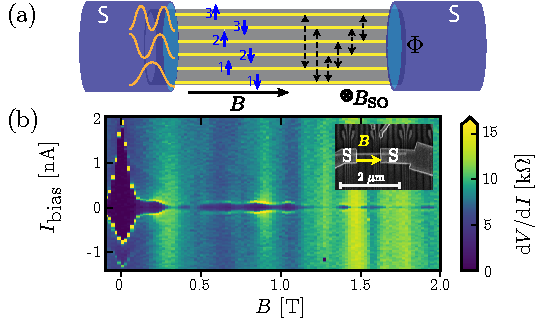
\includegraphics[width=\columnwidth]{figures/fig1.pdf}
\caption{(a) Schematic superconductor ($S$)-nanowire-$S$ Josephson junction. The cross section shows cartoon wave functions of $n=3$ transverse modes and the flux $\Phi$ penetrating the area of the nanowire. The blue arrows indicate spin-resolved modes; the black dashed arrows are same-spin scattering events within the wire. All modes are coupled at the contacts. 
The directions of $B$ and the spin-orbit effective field $B_\mathrm{SO}$ are indicated. (b) Differential resistance $\mathrm{d}V/\mathrm{d}I$ versus $B$ and $I_\mathrm{bias}$.
The current bias sweep direction is from negative to positive. Data from device 1. Inset: SEM image of a typical device similar to those studied here. $S$ labels the superconducting contacts while $B$ indicates the in-plane magnetic field for device 2.}
\label{fig:figure1}
\end{figure}

Figure \ref{fig:figure1}(a) presents a schematic of a few-mode nanowire Josephson junction.
The inset of Fig.~\ref{fig:figure1}(b) shows a device similar to those used in this study and their fabrication process is described in Ref.~\onlinecite{mourik2012signatures}.
The junction consists of an InSb nanowire with a diameter of $100 \pm \SI{10}{nm}$ with 80 nm thick dc magnetron sputtered NbTiN contacts.
The wire sits on top of an array of 50 or $\SI{200}{nm}$ wide gates isolated from the junction by a dielectric. 
We report data from devices 1 and 2 in the main text and show additional data from device 3 in the Supplemental Material, Ref. ~\onlinecite{supp}.
Device 1(2) has a contact spacing of $\sim \SI{1}{\micro \m}$($\sim \SI{625}{nm}$) and the nanowire is at an angle of $25^\circ \pm 5^\circ$($0^\circ \pm 5^\circ$) with respect to $B$. 
Device 3 has a shorter contact spacing of $\sim \SI{150}{nm}$ and shows similar behavior of gate-tunable nodes but the initial critical current decay is extended to 400 mT.
The measurements were performed in a dilution refrigerator with a base temperature of $\sim\SI{60}{mK}$. 
All bias and measurement lines connected to the device are equipped with standard $RC$ and copper powder filtering at the mixing chamber stage to ensure a low electrical noise environment. 
The voltage measurements are performed in the four-terminal geometry.

We set all the gates underneath the nanowire to positive voltages, in the few-mode transparent regime in which no quantum dots are formed between the superconducting contacts, and the normal state conductance exceeds $2e^2/h$ (see the full gate trace of the supercurrent in the Supplemental Material ~\cite{supp}).

Figure \ref{fig:figure1}(b) shows a typical example of the differential resistance $\mathrm{d}V/\mathrm{d}I$ as a function of the magnitude of the magnetic field $B$ and the current bias $I_\mathrm{bias}$ in this few-mode regime, with low resistance supercurrent regions in dark blue around zero current bias. 

Note that the data at low field are asymmetric with respect to current reversal. Only one sweep direction is plotted for the rest of the figures.

A strong decrease of the switching current is observed from $B=\SI{0}{T}$ to $B=100-\SI{200}{mT}$. 
Beyond the initial decrease, the critical current exhibits nonmonotonic behavior with multiple nodes and lobes. 
Despite the \SI{1}{\micro \meter} contact separation, the supercurrent can be resolved up to fields as high as $B=\SI{2}{T}$, which is comparable to the estimated strength of the effective spin-orbit field $B_\mathrm{SO}$.
At finite magnetic fields where the Josephson energy is suppressed the sharp switching behavior is replaced with a smooth transition to a higher resistance state. 
In voltage-biased measurements, this manifests as a zero-bias conductance peak (see Supplemental Material ~\cite{supp}). 
This signal can mimic the onset of the topological phase since it is also associated with the zero-bias conductance peak that appears at a finite magnetic field.

\begin{figure}[t]
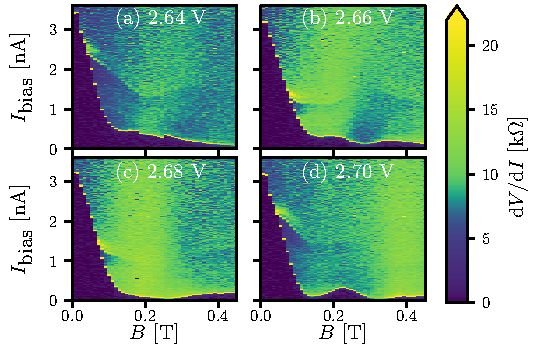
\includegraphics[width=\columnwidth]{figures/fig2.pdf}
\caption{(a)-(d) $\mathrm{d}V/\mathrm{d}I$ vs $B$ and $I_\mathrm{bias}$ for different gate voltage settings $V_\mathrm{g}$ indicated above each panel.  Data from device 2; see the Supplemental Material~\cite{supp} for the scanning electron micrograph of the device with the tuned gate marked.}
\label{fig:figure2}
\end{figure}

We now qualitatively discuss the possible explanations for the behavior observed in Fig. \ref{fig:figure1}(b).
Zeeman splitting can induce $0-\pi$-junction transitions which result in an oscillatory Josephson energy as a function of the magnetic field \cite{bulaevskii1977superconducting,  buzdin1982critical, demler1997superconducting}. 
This alternating $0-\pi$ junction behavior is due to spin-up and spin-down channels acquiring different phases as they travel across the junction [Fig. \ref{fig:figure1}(a)]. 
However, in our junctions a strong spin-orbit effective field, which has been reported to point perpendicular to the nanowire \cite{nadj2012spectroscopy}, reduces the relative phase shifts of spin-up and spin-down and lifts the nodes in the supercurrent\cite{shumeiko2008, yokoyama2014anomalous,yokoyama2014magnetic}.
For the spin-orbit strength previously reported in InSb nanowires \cite{nadj2012spectroscopy, vanweperen2015spinorbit}, we estimate an effective spin-orbit field $B_{\rm SO} \sim 1-\SI{2}{T}$ for a chemical potential value in the middle of the subband.
Therefore, we do not expect the occurrence of $0-\pi$-transitions in ballistic nanowires for fields much lower than this typical value of $B_{\rm SO}$, unless the chemical potential is close to a transverse mode edge (within $1-\SI{2}{meV}$), where $B_{\rm SO}$ is suppressed.
Given the typical mode spacing of $10-\SI{20}{meV}$~\cite{vanweperen2012quantized,kammhuber2016conductance}, in combination with the occurrence of several nodes well below \SI{1}{T}, the Zeeman $\pi$-junction effect is an unlikely explanation for all of the critical current nodes observed here for generic device settings.

Supercurrents carried by different transverse modes would also acquire different phase shifts and interfere due to mode mixing within the wire or at the contact between the nanowire and the superconductor lead~\cite{PhysRevB.91.245436}. 
Such interference is analogous to the Fraunhofer effect in wide uniform junctions: it becomes relevant when a single superconducting flux quantum is threaded through the nanowire cross section, a regime that is reached for $B \approx \SI{0.25}{T}$, well within the range of the present study. 
Comparison of the experimental and numerical data in this Letter suggests that this is the effect that dominates the magnetic field dependence of the critical current.

Transitions in and out of the topological superconducting phase in the nanowire segments covered by the superconductors were also predicted to induce reentrant critical current\cite{san2014mapping}. 
Although we used devices similar to those presented in recent Majorana experiments \cite{mourik2012signatures,Zhang2016ballisticmajoranadevice,chen2016phasediagram}, here we did not gate tune the regions of the wire underneath the superconducting contacts into the topological regime. An accidental topological regime occurring on both sides of the junction in multiple devices is an unlikely explanation for the generic observations reported here. 

Figure~\ref{fig:figure2} shows a typical sequence of magnetic field dependences of the critical current, obtained by adjusting one of the narrow local gates. 
The critical current exhibits multiple nodes [Fig.~\ref{fig:figure2}(d)], just a single node [Fig.~\ref{fig:figure2}(c)], or no node [Fig.~\ref{fig:figure2}(a)] in the same field range.
At some nodes the critical current goes to zero, while a nonzero supercurrent is observed at other nodes. 
No periodic patterns such as those characteristic of a dc-SQUID or a uniform junction are observed. 
Note that slight changes in the gate voltage are sufficient to dramatically alter the magnetic field evolution curve; the corresponding change in chemical potential $\Delta \mu$ is small ($\Delta \mu < \SI{1}{\milli \electronvolt}$) compared with the typical intermode spacing ($\sim \SI{15}{\milli \electronvolt}$). 
Furthermore, the gate used only tunes a \SI{100}{\nano \meter} segment of the \SI{650}{\nano \meter} long junction.

Typical gate sweeps of the supercurrent are presented in Fig.~\ref{fig:figure3}. 
The critical current is strongly reduced at fields above \SI{100}{\milli \tesla} irrespective of the gate voltage. 
At all fields, the supercurrent is strongly modulated by the gate voltage. 
However, gate voltages at which nodes in the critical current occur differ for each magnetic field. 
Thus, no straightforward connection can be made between the zero-field critical current and node positions at a finite field, see also Fig.~\ref{fig:figure5}(a). 

\begin{figure}
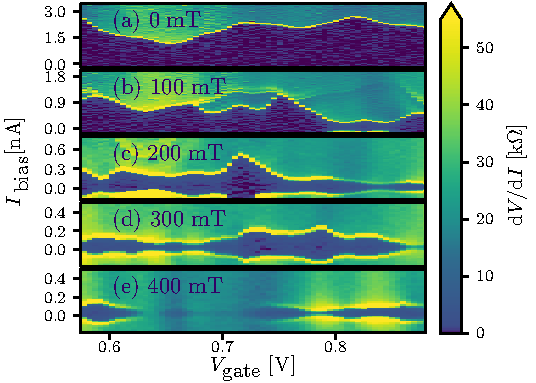
\includegraphics[width=\columnwidth]{figures/fig3.pdf}
\caption{(a)-(e) $\mathrm{d}V/\mathrm{d}I$ vs $V_\mathrm{g}$ and $I_\mathrm{bias}$ at different $B$ (indicated within each panel). Data from device 2. The gate used for tuning is different from that used in Fig.~\ref{fig:figure2}, see the Supplemental Material~\cite{supp}. }
\label{fig:figure3}
\end{figure}

\begin{figure*}[t]
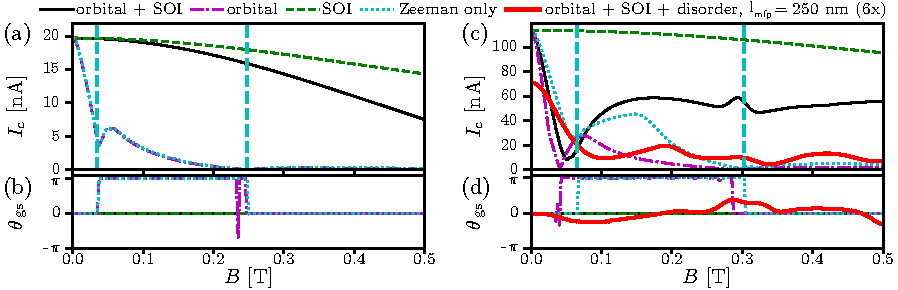
\includegraphics[width=\textwidth]{fig4.pdf}
\caption{Critical current and corresponding ground state phase difference for different combinations of terms in the Hamiltonian.
The Zeeman effect ($g=50$) is present in all of the curves.
Only the system corresponding to the red curve labeled with $l_\textrm{mfp}=\SI{250}{nm}$ includes disorder, for which the critical current is multiplied by a factor of 6. The simulation is performed at $T=\SI{100}{mK}$.
The curves in panels (a) and (b) are for a single spinful transverse mode ($\mu=\SI{10}{meV}$).
Panels (c) and (d) are for the multimode (three transverse or six spin-full modes) regime ($\mu=\SI{20}{meV}$).
The vertical thick dashed light blue lines in (a) and (c) indicate the positions of $0-\pi$ transitions in the absence of disorder and with $\alpha = 0$, $\bm{A}=0$.
Where not specified, the other constant simulation parameters are $\alpha=\SI{20}{\nm \meV}$, $m_\textrm{eff}=0.015 m_\textrm{e}$, $\Delta_\textrm{ind}=\SI{0.250}{meV}$; the lattice constant $a=\SI{8}{nm}$, the nanowire diameter $d_1=\SI{104}{nm}$, the outer diameter (with superconductor) $d_2=\SI{120}{nm}$, and the superconductor coverage angle (see the Supplemental Material~\cite{supp}, Fig.6) $\phi=135\si{\degree}$. For plots of corresponding current-phase relationships, Josephson energies, and numerical geometry, see the Supplemental Material ~\cite{supp}, Fig. 6-9.
}
\label{fig:critical_currents}
\end{figure*}

In order to understand the magnetic field evolution of the Josephson effect, we develop an effective low-energy model of a spin-orbit and Zeeman-coupled few-mode nanowire, covered by superconductors at both ends. 
We define $x$ as the direction along the wire, $y$ perpendicular to the wire in the plane of the substrate, and $z$ perpendicular to both wire and substrate. 
The corresponding Hamiltonian reads
\begin{align}
H = &\left(\frac{\bm{p}^2}{2m^*}-\mu + \delta U\right)\tau_z + \alpha (p_x \sigma_y - p_y \sigma_x)\tau_z \nonumber \\ &+ g \mu_B \bm{B}\cdot\boldsymbol{\sigma} + \Delta \tau_x. 
\label{eq:H}
\end{align}
Here $\bm{p}=-i\hbar\nabla+e\bm{A}\tau_z$  is the canonical momentum,  where $e$ is the electron charge, and $\bm{A}={\left[ B_y z - B_z y,\; 0,\; B_x y\right]}^{T}$ is the vector potential chosen such that it does not depend on $x$. 
Further, $m^*$ is the effective mass, $\mu$ is the chemical potential controlling the number of occupied subbands in the wire, $\alpha$ is the strength of Rashba spin-orbit interaction, $g$ is the Land{\'e} $g$-factor, $\mu_\mathrm{B}$ is the Bohr magneton, and $\Delta$ is the superconducting pairing potential.
The Pauli matrices $\sigma_i$ and $\tau_i$ act in spin and electron-hole spaces, respectively.
We assume that the electric field generated by the substrate points along the $z$ direction, such that the Rashba spin orbit acts in the $xy$\kern-.05ex-plane, which is at low energies equivalent to an effective magnetic field $\bm{B}_{\rm SO}\parallel\hat{y}$.
We include the vector potential in the tight-binding system using the Peierls substitution \cite{hofstadter_energy_1976}.
Finally, we include an uncorrelated on-site disorder $\delta U \in [-U, U]$, with $U$ the disorder strength, which we parametrize by a normal state mean free path $l_\textrm{mfp}$. \cite{beenakker1997random}$^\textrm{,}$\footnote{To determine $l_\textrm{mfp}$ we calculate a disorder-averaged normal state conductance $g$ and evaluate the mean free path $l_{mfp}$ by fitting, $g=g_0 N_\textrm{ch} / (1 + L / l_\textrm{mfp})$, with $N_\textrm{ch}$ the number of conduction channels, and $g_0$ conductance quantum.}

We perform numerical simulations of the Hamiltonian \eqref{eq:H} on a 3D lattice in a realistic nanowire Josephson junction geometry. 
The critical current is calculated using the algorithm described in Ref.~\onlinecite{ostroukh2016two} and the Kwant code \cite{groth_kwant}.
We note that for moderately damped and overdamped Josephson junctions, such as those studied here, the theoretical $I_c$ closely follows the experimentally measured switching current \cite{kautz1990noise}. 
The source code and the specific parameter values are available in the Supplemental Material ~\cite{supp}.
The full set of materials, including computed raw data and experimental data, is available in Ref.~\onlinecite{data}.

Numerical results are presented in Figs. \ref{fig:critical_currents} and \ref{fig:figure5}(b).
First, we discuss the case of only a single transverse mode occupied [Figs.~\ref{fig:critical_currents}(a) and ~\ref{fig:critical_currents}(b)], which is pedagogical but does not correspond to the experimental regime.
When all field-related terms of Eq.~\eqref{eq:H} are included ($\bm{A}\neq 0$, $\alpha \neq 0$), we observe a monotonic decay of the critical current much more gradual than in the experiment, due to the absence of the intermode interference effect in the single-mode regime.
The $\pi$-junction transitions do not appear up to fields of order $\SI{0.5}{T}$ due to the strong spin-orbit effective field, which keeps spin-up and spin-down at the same energy so that they acquire the same phase shifts traversing the junction.
The critical current eventually decays because the Zeeman term overtakes the spin-orbit term at fields greater than \SI{0.5}{\tesla}. 
When the spin-orbit term is turned off ($\alpha = 0$), we see several $0-\pi$ transitions taking place within the studied field range, confirmed by the ground state phase switching between 0 and $\pi$ at a series of magnetic fields [Fig.~\ref{fig:critical_currents}(b)].

The experimentally relevant regime is when several transverse modes are occupied. 
The measurements display three qualitative features: (i) the initial critical current at $B=\SI{0}{T}$ is strongly suppressed within $100-200$mT; (ii) the critical current then revives and continues to display nodes of variable depth and periodicity; (iii) this revival of the critical current after suppression is about 10\% of its original value at $B=\SI{0}{T}$.
Models that neglect the orbital effect display either a slow monotonic decay of the critical current (spin-orbit included, $\alpha \neq 0$), or regular critical current nodes due to $0-\pi$ transitions (no spin-orbit, $\alpha=0$) [Fig.~\ref{fig:critical_currents}(d)], as in the single-mode case.
When orbital effects are included, $\bm{A}\neq 0$, observations (i) and (ii) are reproduced but the revival of the critical current after initial suppression is still strong.
Inclusion of a realistic amount of disorder, which creates additional interference paths and suppresses supercurrent further, reproduces all observations (i), (ii), and (iii).
Thus, we conclude that the experiment is best reproduced when $\bm{A}\neq 0, \alpha \neq 0$ and weak disorder that induces intermode scattering is included within the junction model.

The inclusion of disorder in the multimode regime breaks mirror symmetry~\cite{yokoyama2014anomalous,yokoyama2014magnetic} and generates a spin-orbit field along the external magnetic field \textit{B}, which gives rise to a nonsymmetric current-phase relation, inducing a $\varphi_0$ junction (see the Supplemental Material ~\cite{supp}, Sec. VIII, for a detailed explanation). 
The ground state phase of the $\varphi_0$ junction can continuously change between 0 and $\pi$ [red trace in Fig.~\ref{fig:critical_currents}(d)]. 
Experimental verification of such phase-related effects is not possible in the two-terminal junction geometry used here, it requires phase-sensitive experiments in the SQUID geometry.

\begin{figure}[t]
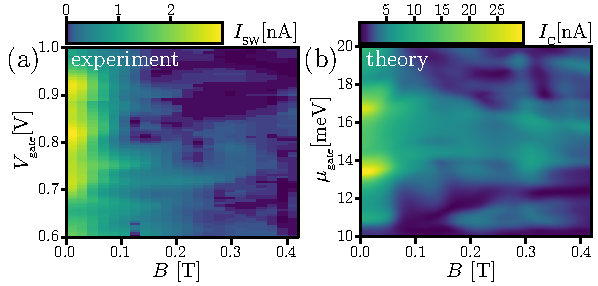
\includegraphics[width=\columnwidth]{figures/fig5.pdf}
\caption{Comparison between experimental (a) and numerical (b) results.
The parameters for the numerical simulations are the same as in Figs. \ref{fig:critical_currents}(c) and \ref{fig:critical_currents}(d), red curve.
The range of the chemical potential in the gated region ($\mu_{\textrm{gate}}$) is chosen using Ref. \onlinecite{vuik}. The experimental data are taken with device 2.}
\label{fig:figure5}
\end{figure}

In Fig.~\ref{fig:figure5} we compare side-by-side experiment and simulations via field-versus-gate maps of the supercurrent. 
In Fig.~\ref{fig:figure5}(a), the switching current from a set of $\mathrm{d}V/\mathrm{d}I$ vs. $I_\textrm{bias}$ traces similar to those in Fig.~\ref{fig:figure3} was extracted from device 2 (see the Supplemental Material ~\cite{supp} for algorithm details). 
Beyond the decay of the switching current on the scale of $\SI{100}{mT}$, the experimental data show a complex evolution of switching current maxima and minima in gate-field space. 
Characteristic features of this evolution are reproduced by our simulation shown in Fig.~\ref{fig:figure5}(b).
In particular, the experimentally observed magnetic field scale of initial supercurrent decay is reproduced in the simulation.
Furthermore, the gate-tunable maxima and minima of the critical current are recovered in our model; both in experiment and simulation these do not evolve in a regular fashion (a consequence of the complexly shaped interference trajectories). 
This qualitative agreement found additionally substantiates the applicability of our model to the experimental results.

Our results are instrumental for modeling Majorana setups. 
Specifically, the decrease of Josephson energy by an order of magnitude is observed at fields at which the onset of topological superconductivity is reported. 
This effect should, therefore, be taken into account in efforts to realize recent proposals for fusion and braiding of Majorana fermions \cite{Hyart2013braiding, Aasen2016briading, plugge2016majorana, Karzig2016braiding}, especially in those that rely on controlling the Josephson coupling \cite{Hyart2013braiding, Aasen2016briading, plugge2016majorana}. 
Our findings are applicable not only to bottom-up grown nanowires and networks but also to scalable few-mode junctions fabricated out of two-dimensional electron gases. \cite{nichelle2017scalingzbp,lee2017inas2deg} 
We suggest that in such devices narrow multimode nanowires should be used. 
At the magnetic field strengths required for braiding the many modes would facilitate strong Josephson coupling, whereas a small diameter prevents its suppression due to supercurrent interference.

Phase-sensitive measurements in the SQUID loop geometry will reveal effects  such as the Zeeman-induced  $\pi$ junction and the spin-orbit induced $\varphi_0$ junction, which our study identifies numerically but does not access experimentally. 
Single quantum mode junctions are within reach thanks to the recent demonstration of quantum point contacts in InSb nanowires at a zero magnetic field \cite{kammhuber2016conductance}. 
In that regime phenomena such as induced $p$-wave superconductivity can be studied in a unique gate-tunable setup, when tuning down to a single spin-polarized mode in the weak link. 
The results are also applicable to other interesting material systems where spin-orbit, orbital,  and Zeeman effects interplay - systems such as Ge/Si, PbS, InAs, and  Bi nanowires and carbon nanotubes. \cite{cleuziou2006carbon}

\textit{Acknowledgments.} This work has been supported by the European Research Council, the Netherlands Organization for Scientific Research (NWO), the Foundation for Fundamental Research on Matter (FOM), and Microsoft Corporation Station Q.
V.M. was supported by a Niels Stensen Fellowship for part of the research. 
A.R.A., D.I.P., and S.M.F. are grateful to KITP, where part of the research was conducted with the support of NSF Grant No. PHY11-25915. S.M.F acknowledges NSF Grant No. DMR-125296, S.M.F., L.P.K. and E.P.A.M.B. acknowledge ONR. 
D.I.P. thanks NSERC, CIFAR, and the Max Planck - UBC Centre for Quantum Materials for support.

\bibliography{bibliography.bib}

\end{document}
